% !TEX root = ../../hw01.tex
% Homework 01, Exercise 1. Shared solution.

% Transcribed from IMG_8995 and the left page of IMG_8996.
\begin{proof}[Solution]
Fix a set $S$ such that $A_\gamma\subseteq S$ for every
$\gamma\in\Gamma$. All complements in this proof are taken
relative to $S$, so
\[
  A_\gamma^c=S\setminus A_\gamma.
\]
Suppose first that $\Gamma$ is nonempty. We prove each identity
by showing both inclusions.

\begin{marginfigure}
  \centering
  % !TEX root = ../../problems/hw01.tex
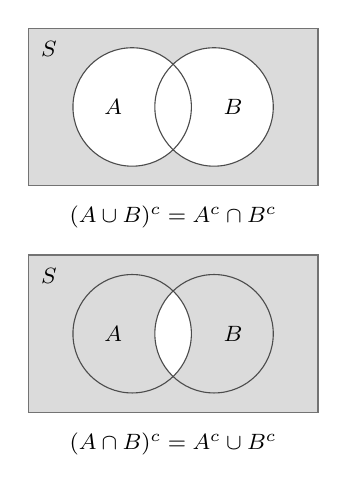
\begin{tikzpicture}[x=0.8cm,y=0.8cm,font=\footnotesize]
  \foreach \offset in {0,-3.6} {
    \begin{scope}[shift={(0,\offset)}]
      \fill[black!14] (0,0) rectangle (4.6,2.5);
    \end{scope}
  }
  % Removing both discs leaves the complement of their union.
  \fill[white] (1.65,1.25) circle[radius=0.94];
  \fill[white] (2.95,1.25) circle[radius=0.94];
  % Removing only the lens leaves the complement of the intersection.
  \begin{scope}[shift={(0,-3.6)}]
    \clip (1.65,1.25) circle[radius=0.94];
    \fill[white] (2.95,1.25) circle[radius=0.94];
  \end{scope}
  \foreach \offset in {0,-3.6} {
    \begin{scope}[shift={(0,\offset)}]
      \draw[black!55] (0,0) rectangle (4.6,2.5);
      \draw[black!70] (1.65,1.25) circle[radius=0.94];
      \draw[black!70] (2.95,1.25) circle[radius=0.94];
      \node at (1.35,1.25) {$A$};
      \node at (3.25,1.25) {$B$};
      \node[anchor=north west] at (0.05,2.45) {$S$};
    \end{scope}
  }
  \node at (2.3,-0.5) {$(A\cup B)^c=A^c\cap B^c$};
  \node at (2.3,-4.1) {$(A\cap B)^c=A^c\cup B^c$};
\end{tikzpicture}

  \caption[De Morgan's laws.]{The upper shaded region lies outside both sets.
    In the lower panel, only the overlap is excluded. All complements
    are taken within the rectangle $S$.}
  \label{fig:hw01:de-morgan}
\end{marginfigure}

\textit{The complement of the union.}
Suppose that
\[
  x\in\left(\bigcup_{\gamma\in\Gamma}A_\gamma\right)^c.
\]
Then $x\in S$ and $x$ does not belong to the union.
If $x$ belonged to any $A_\gamma$, it would belong to the union.
Therefore $x\notin A_\gamma$ for every $\gamma\in\Gamma$.
Since $x\in S$, this gives $x\in A_\gamma^c$ for every $\gamma$,
and hence
\[
  x\in\bigcap_{\gamma\in\Gamma}A_\gamma^c.
\]

Conversely, suppose that
\[
  x\in\bigcap_{\gamma\in\Gamma}A_\gamma^c.
\]
Then $x\in S$ and $x\notin A_\gamma$ for every $\gamma\in\Gamma$.
Thus no member of the family contains $x$, so $x$ does not belong
to their union. Consequently,
\[
  x\in\left(\bigcup_{\gamma\in\Gamma}A_\gamma\right)^c.
\]
Both inclusions hold, proving the first equality.

\handoutonly{\clearpage}

\textit{The complement of the intersection.}
Suppose that
\[
  x\in\left(\bigcap_{\gamma\in\Gamma}A_\gamma\right)^c.
\]
Then $x\in S$ and $x$ does not belong to the intersection.
There must be an index $\gamma_0\in\Gamma$ for which
$x\notin A_{\gamma_0}$. Otherwise, $x$ would belong to every
$A_\gamma$ and therefore to their intersection.
Thus $x\in A_{\gamma_0}^c$, which gives
\[
  x\in\bigcup_{\gamma\in\Gamma}A_\gamma^c.
\]

Conversely, suppose that
\[
  x\in\bigcup_{\gamma\in\Gamma}A_\gamma^c.
\]
Then $x\in A_{\gamma_0}^c$ for at least one index $\gamma_0$.
Hence $x\in S$ and $x\notin A_{\gamma_0}$.
Since $x$ fails to belong to this member of the family, it cannot
belong to the intersection. Thus
\[
  x\in\left(\bigcap_{\gamma\in\Gamma}A_\gamma\right)^c.
\]
Both inclusions hold, proving the second equality.

If $\Gamma$ is empty, we use the relative conventions
\[
  \begin{aligned}
    \bigcup_{\gamma\in\varnothing}A_\gamma&=\varnothing,\\
    \bigcap_{\gamma\in\varnothing}A_\gamma&=S.
  \end{aligned}
\]
Both identities then follow from $\varnothing^c=S$ and $S^c=\varnothing$.

\autoref{fig:hw01:de-morgan} illustrates the difference for two sets.
An element outside their intersection may still belong to one
of the sets. It simply cannot belong to both.
\end{proof}
